% Software Development for Mobile Devices
\documentclass[11pt,english,numbers=endperiod,parskip=half]{scrartcl}

\usepackage{color}
\usepackage{graphicx}
\usepackage{minted}
\usepackage{fancyhdr}
\usepackage{pdflscape}
\usepackage[final]{pdfpages}
\usepackage{harvard}

\pagestyle{fancy}

\rhead{Daniel Parker - 971328X}
\lhead{COS30017 - Software Development for Mobile Devices}

\title{Assignment 07}
\subtitle{COS30017 - Software Development for Mobile Devices}
\author{Daniel Parker 971328X}

\date{\today}

\begin{document}
\maketitle
\thispagestyle{empty}

\section{Introduction}
	This report outlines the process and findings from completing a usability study
	on a smartphone application. The application is named `Suntime' and allows users
	to get the sunrise and sunset times for a specified location and date. The
	purpose of the usability test is to find any glaring issues with the design of
	the user interface and also to get feedback from possible users about how easy
	the app is to use. The results showed that overall the app was not too
	difficult	too use, however some aspects of the UI could be clearer.
\section{Usability Test Method}
	The usability test was conducted as per the assignment handout. The handouts,
	survey and results sheet used have been attached in the appendix.

	\begin{enumerate}
		\item{
			Tester is provided with the information sheet covering the app
			and usability test information to read. The tester is instructed to read all
			the information
		}

		\item{
			The tester is asked to complete each scenario using the prototype app and
			reminded to verbalise what they are doing and to give any feedback as they
			are completing the scenario.
		}

		\item{
			During the completion of the scenarios the supervisor records all the
			comments made by the user and also what difficulties they have. The
			supervisor cannot give assistance, however they can act as the phone's
			GPS sensor when appropriate.
		}

		\item{
			If the tester is unable to complete the scenario, record it and any further
			information as to why they were stuck.
		}

		\item{
			After all the scenarios have been completed / attempted, the tester is
			provided with a short questionnaire to complete.
		}

		The participants are referred to as P1 - P3 to retain anonymity.
	\end{enumerate}

\section{Findings}
	From the questionnaire results, it's observed that tester P1 feels that the UI
	does not communicate clearly to them how to complete a given scenario. Tester
	P2 feels that the layout and functionality of the application is not
	very effective. All testers felt that the prototype was visually clear and
	that readability was good.

	Questions 4 and 5 brought low reviews from users P1 and P2, indicating that it
	was difficult to complete some of the scenarios on the prototype, and also
	that the prototype didn't communicate the app's intent very well. User P2
	commented that the app has too much `drill-down', which means that there are
	too many screens that need to be navigated through to get to the desired
	information. This is backed up by a comment from P3 that perhaps the preset
	locations should be shown on the landing / home screen instead of buttons to
	access the three different location types.

\section{Discussion}
	This usability test has yielded some interesting and unexpected results. The
	testers have given huge insight into the true usability of the prototype, and
	valuable feedback on what should be changed. In particular the first tester P1
	had quite a bit of trouble in scenario 1. It took them over 2 minutes to find
	the $+$ icon on the custom locations screen.

	All the testers had trouble finding the correct share icon to use
	when trying to share suntime information for a range of dates. All testers
	navigated to a specific day and shared from that screen instead of the date
	range screen. This suggests that it's not clear what the share icon does in
	this context, and also that perhaps	having it available on two adjacent
	screens creates some confusion about what is being shared.

	Across all three participants, it was observed that they had to enter various
	parts of the app, before realising that it wasn't what they were trying to
	achieve, and then use the back-button convention to return and try another
	option. This further supports the comments of two of the participants that
	there is too much drill-down in the application's navigation.

	Following the usability test, the following aspects of the design will be
	changed;
	\begin{itemize}
		\item{
			The preset locations will be moved to be the home screen, and new
			action-bar navigation will be added to support the current location and
			custom location features. \cite{phandroid}
		}

		\item{
			The share buttons will remain where they are, however the share button on
			the individual day screen will show a dialog box that asks whether the
			user would like to share just that day or every day in the range given.
		}
	\end{itemize}

	I have learnt from doing this usability test that a prototype which I have
	designed myself, and appears to be easy to use and clear, is not necessarily
	clear to use for someone else. Most of the difficulties that testers had with
	that app were navigation related and have given me insight into the concept of
	having less complex drill-down to avoid confusing the user. \cite{msdn}

\section{Summary}
This usability test has shown some usability issues in the `Suntime' prototype.
The participants found it difficult to navigate to the part of the app they
needed to complete a given task, and also consistently misused the share icon in
the app. These issues will be taken into account when simplifying the design.
A lot has been learnt regarding the reasons for conducting usability tests on
an app design. The importance of usability testing in creating effective and
usable apps is high and has contributed to improving the UI of the `Suntime' app.

\bibliography{references}{}
\bibliographystyle{agsm}

\section{Appendix}
	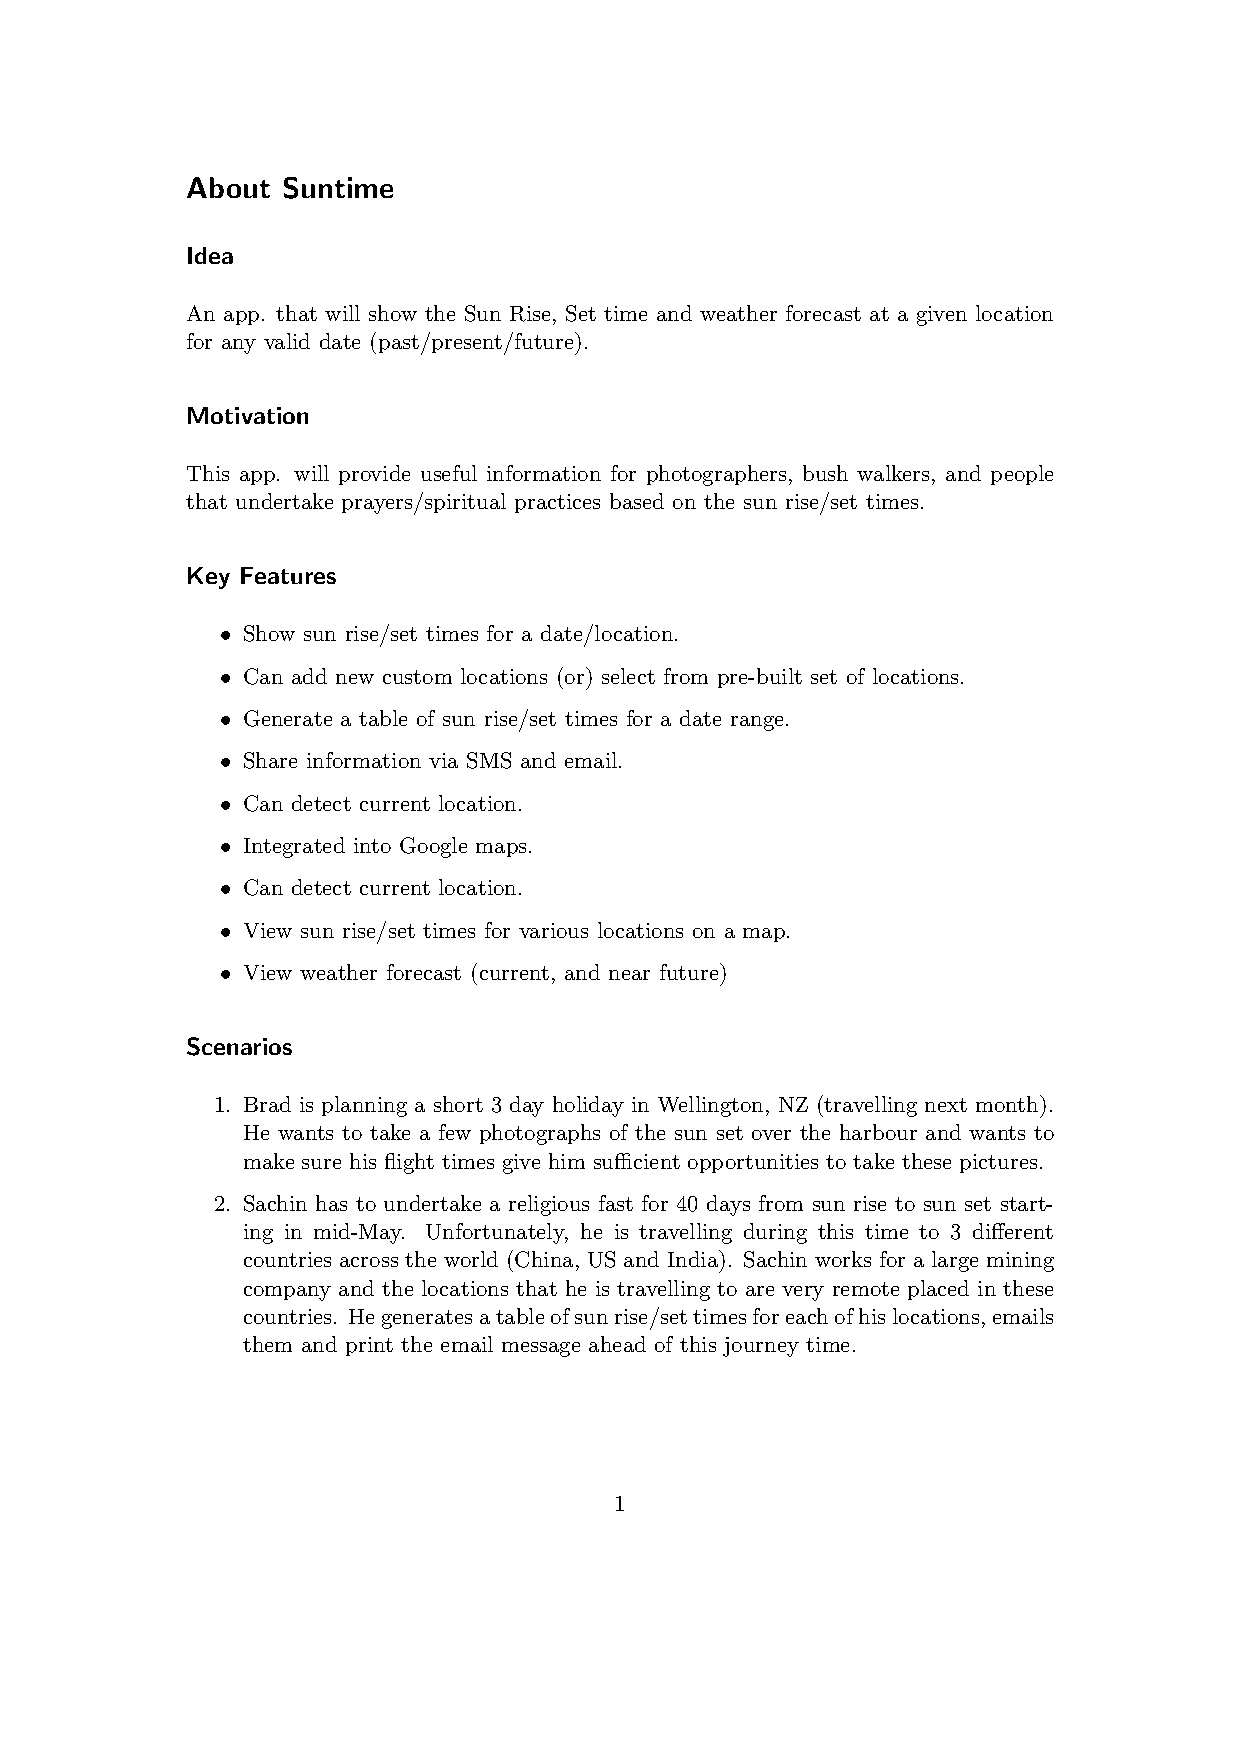
\includepdf[pages=1-2]{info.pdf}
	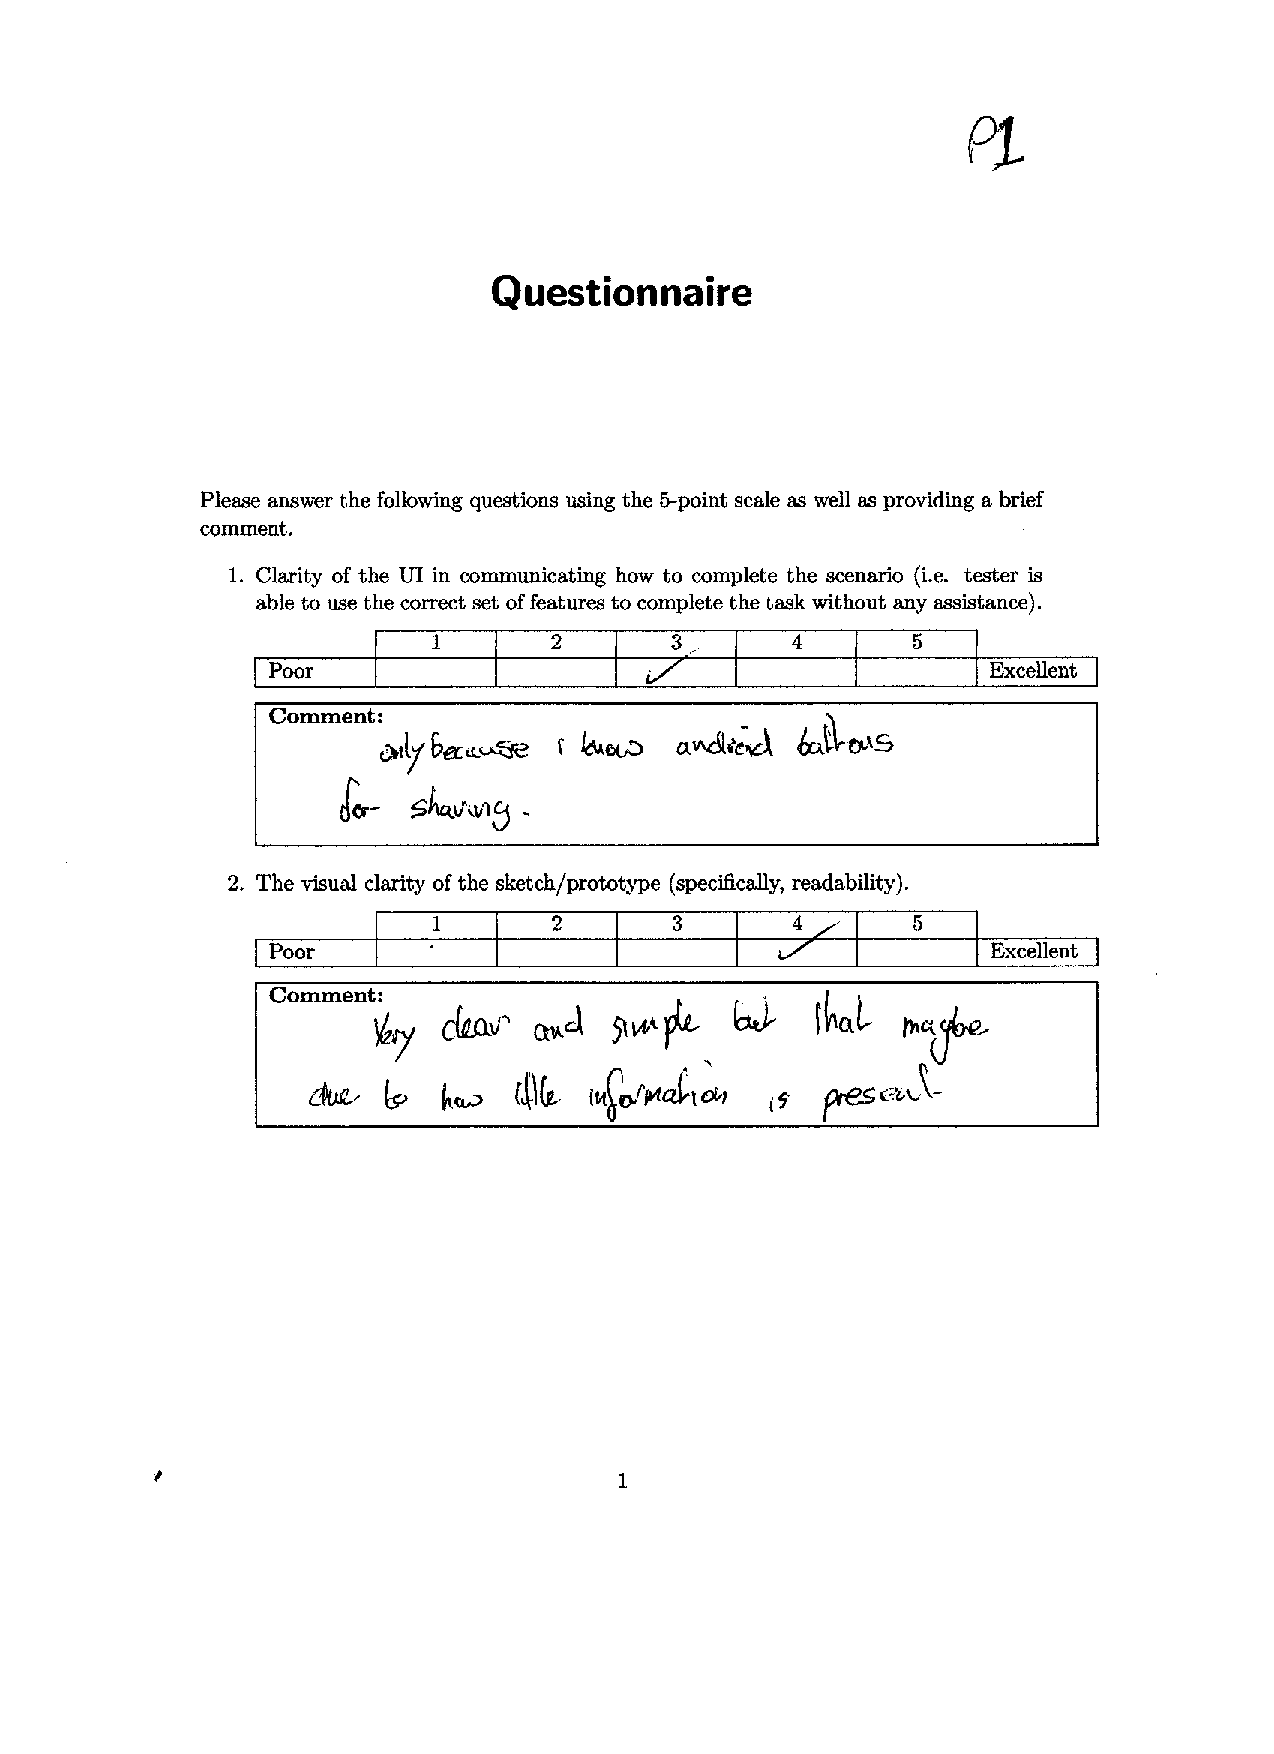
\includepdf[pages=1-2]{Results/P1-Q.pdf}
	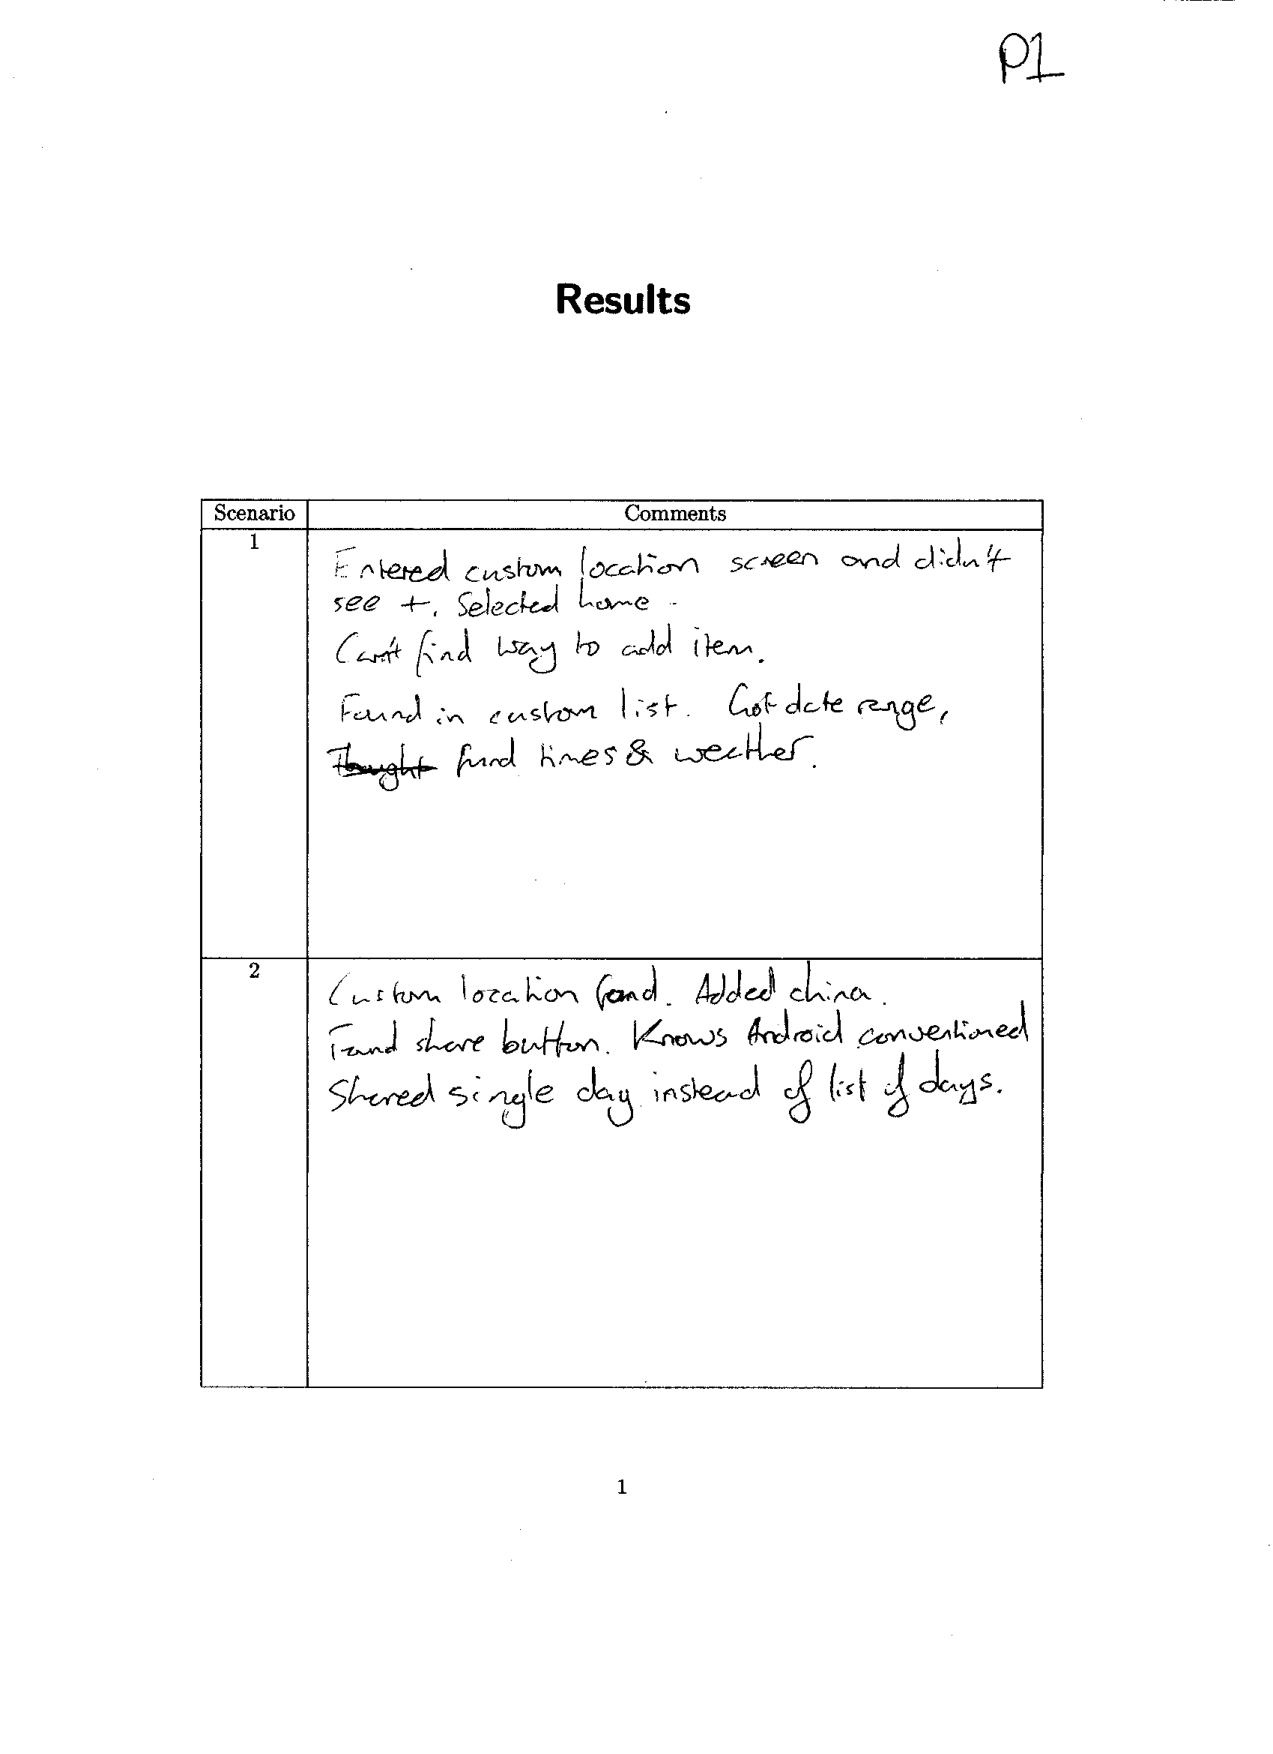
\includepdf[pages=1-2]{Results/P1-R.pdf}
	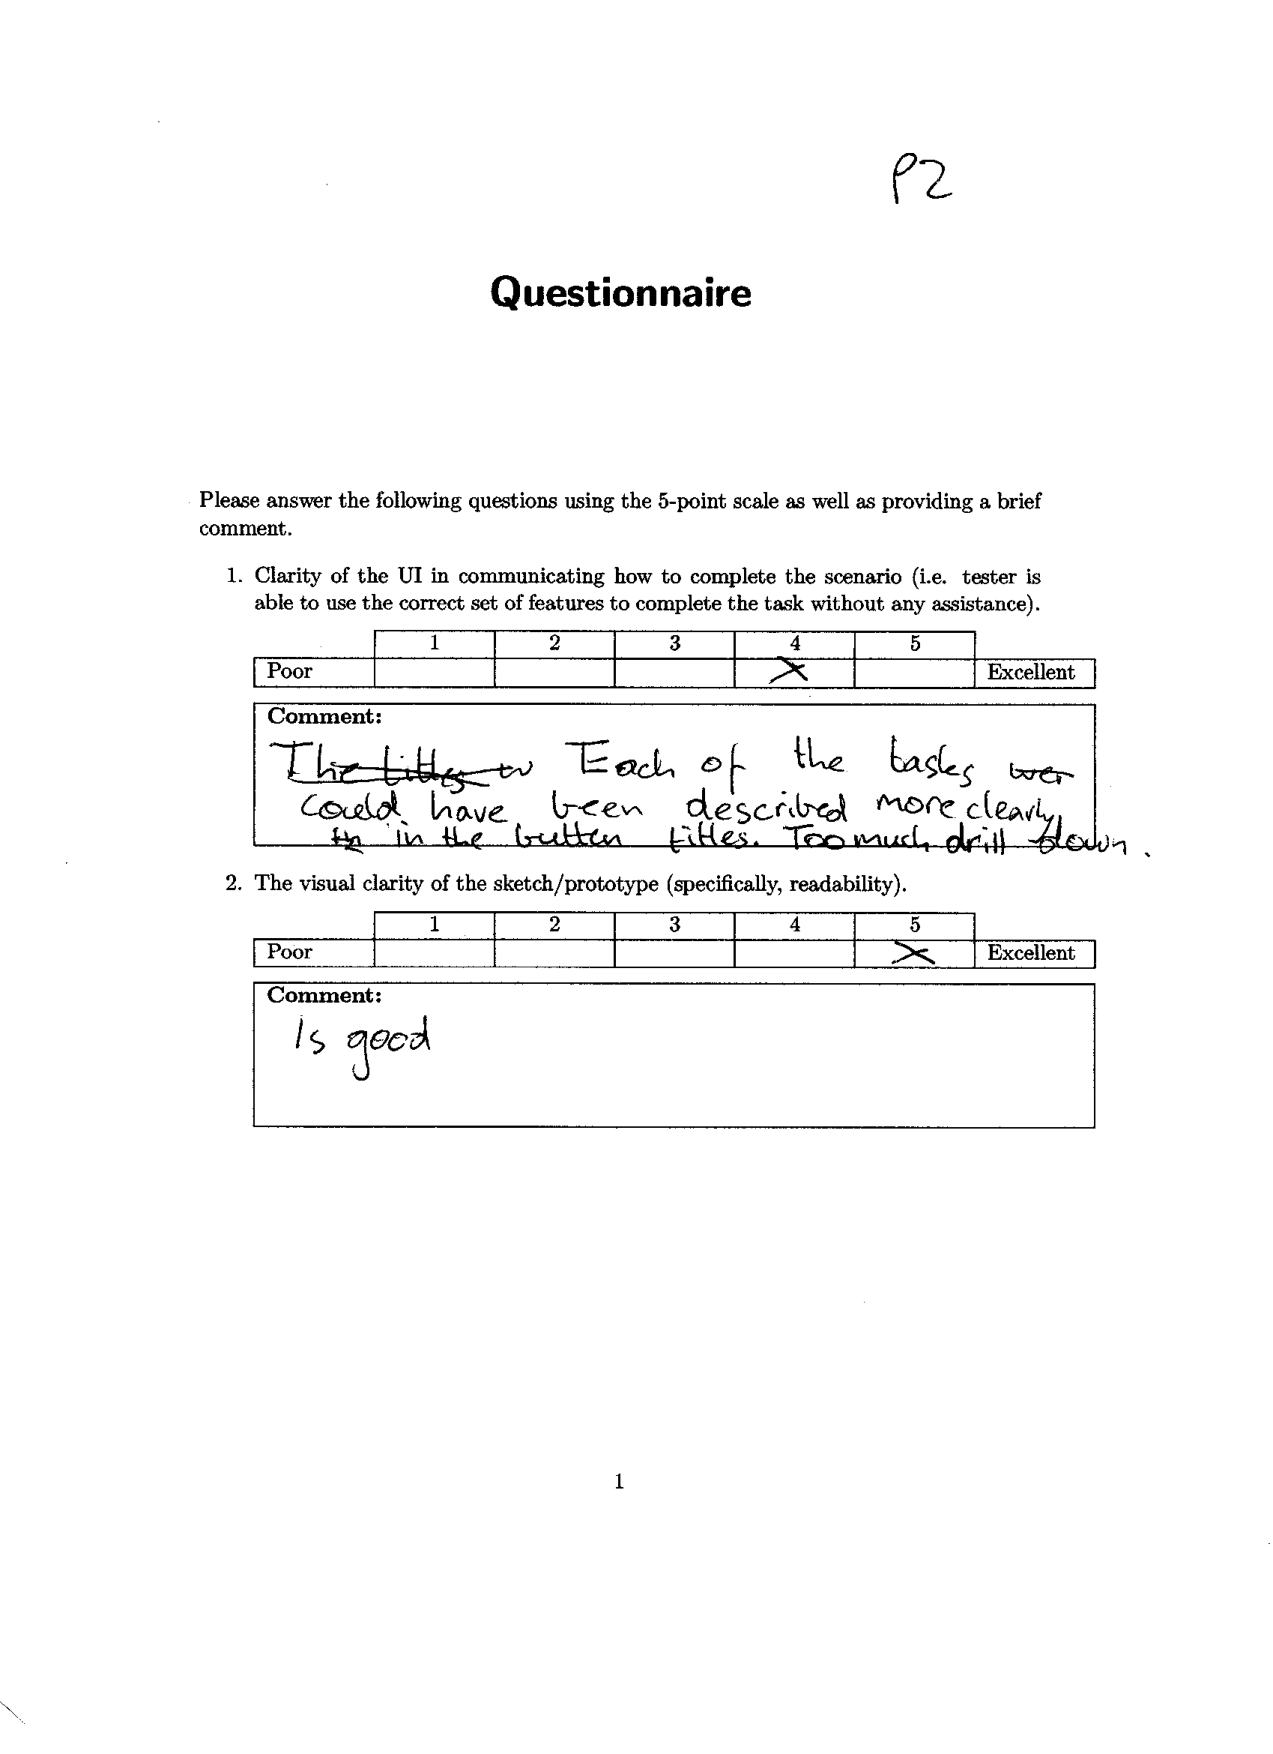
\includepdf[pages=1-2]{Results/P2-Q.pdf}
	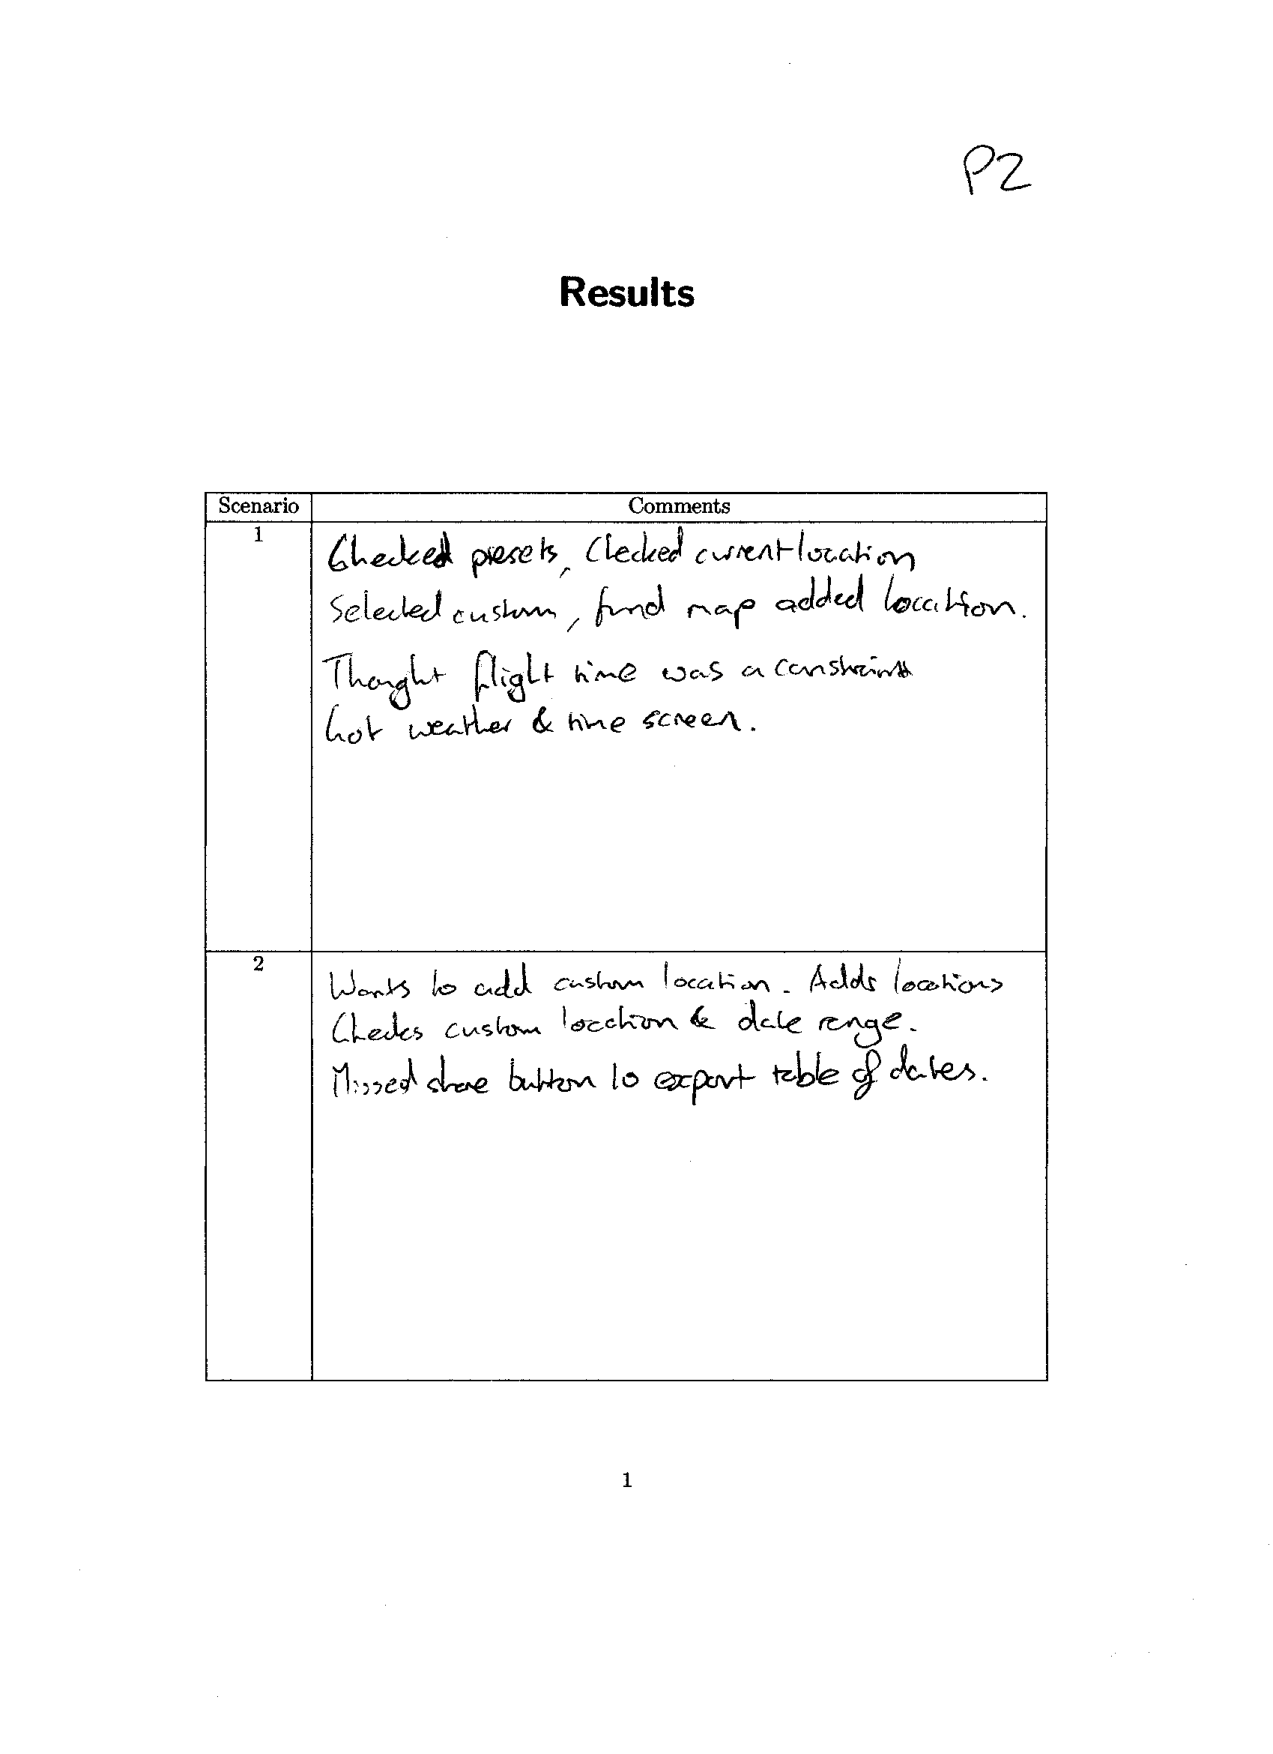
\includepdf[pages=1-2]{Results/P2-R.pdf}
	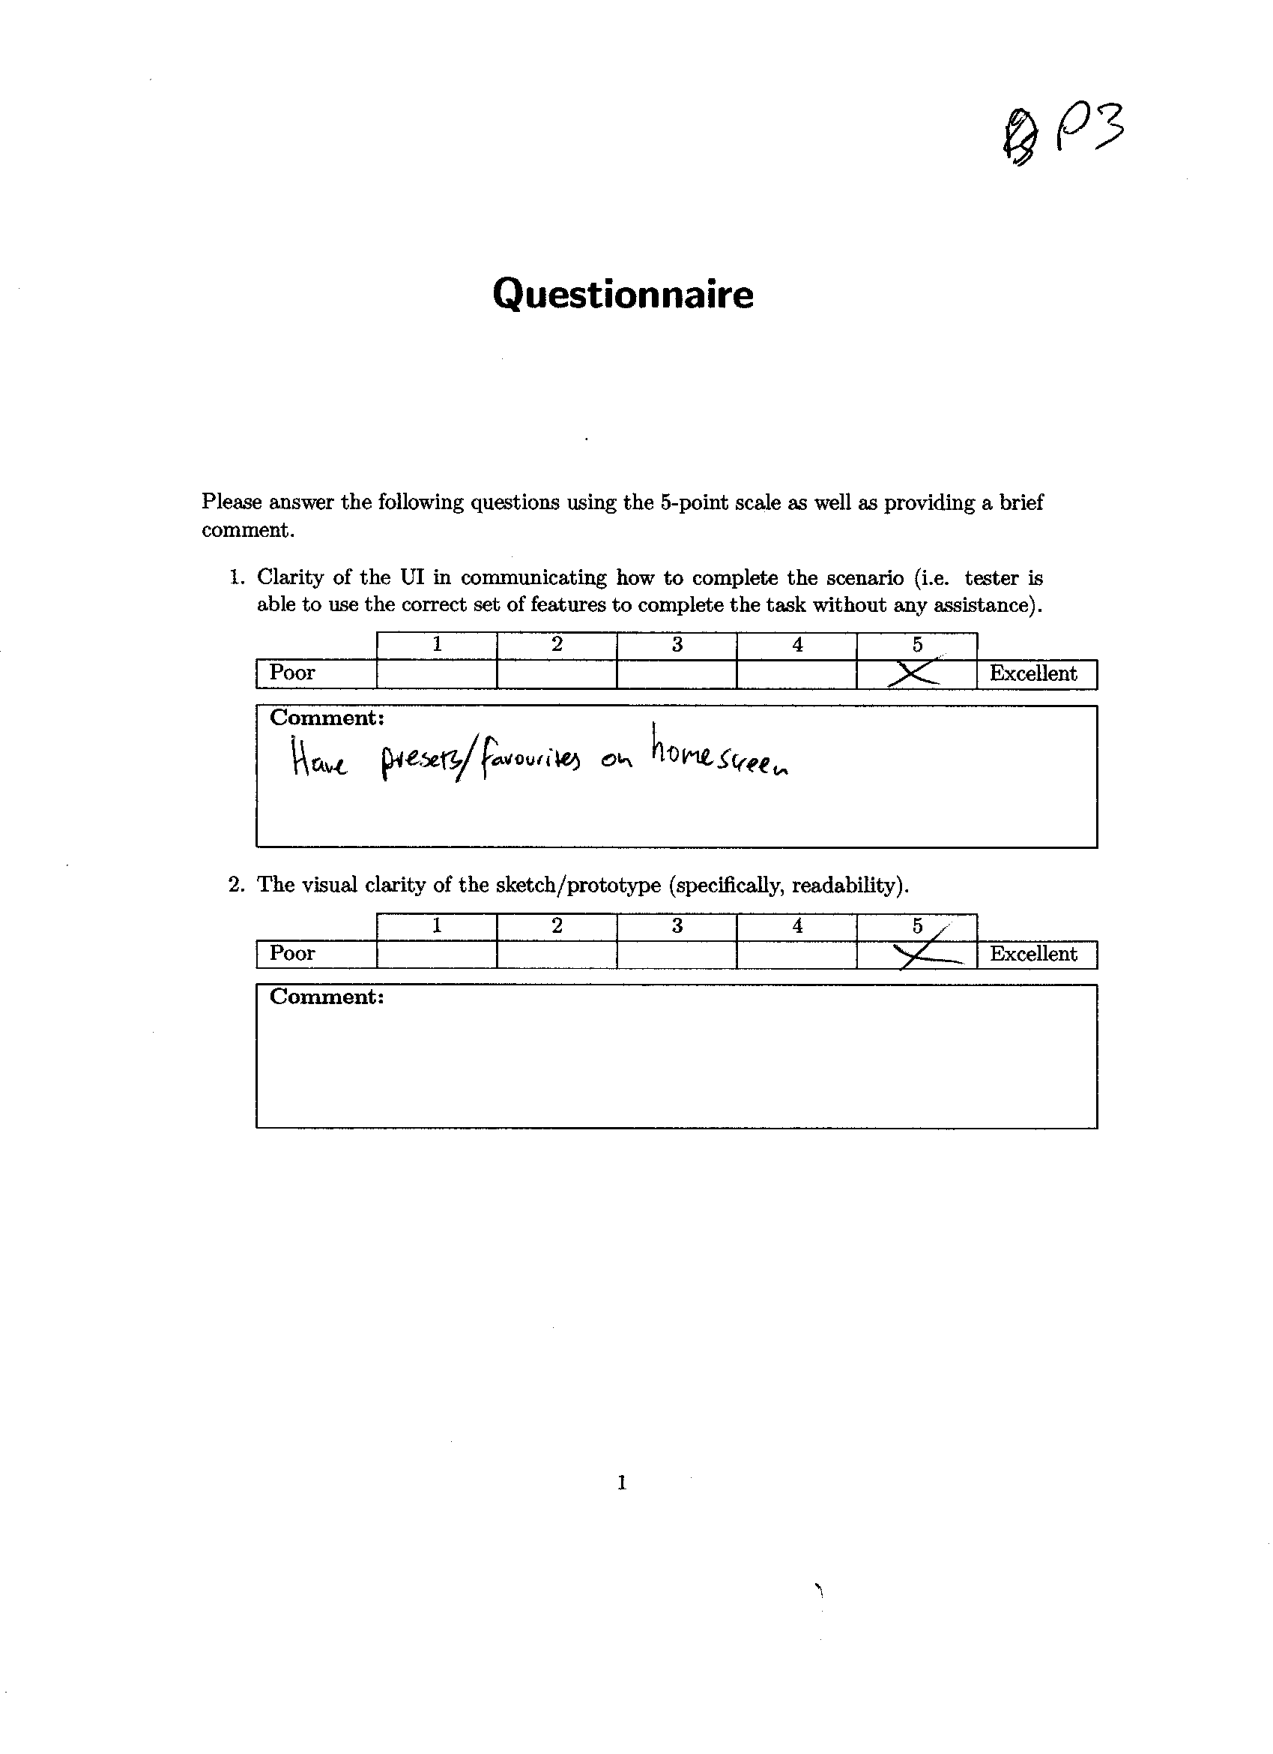
\includepdf[pages=1-2]{Results/P3-Q.pdf}
	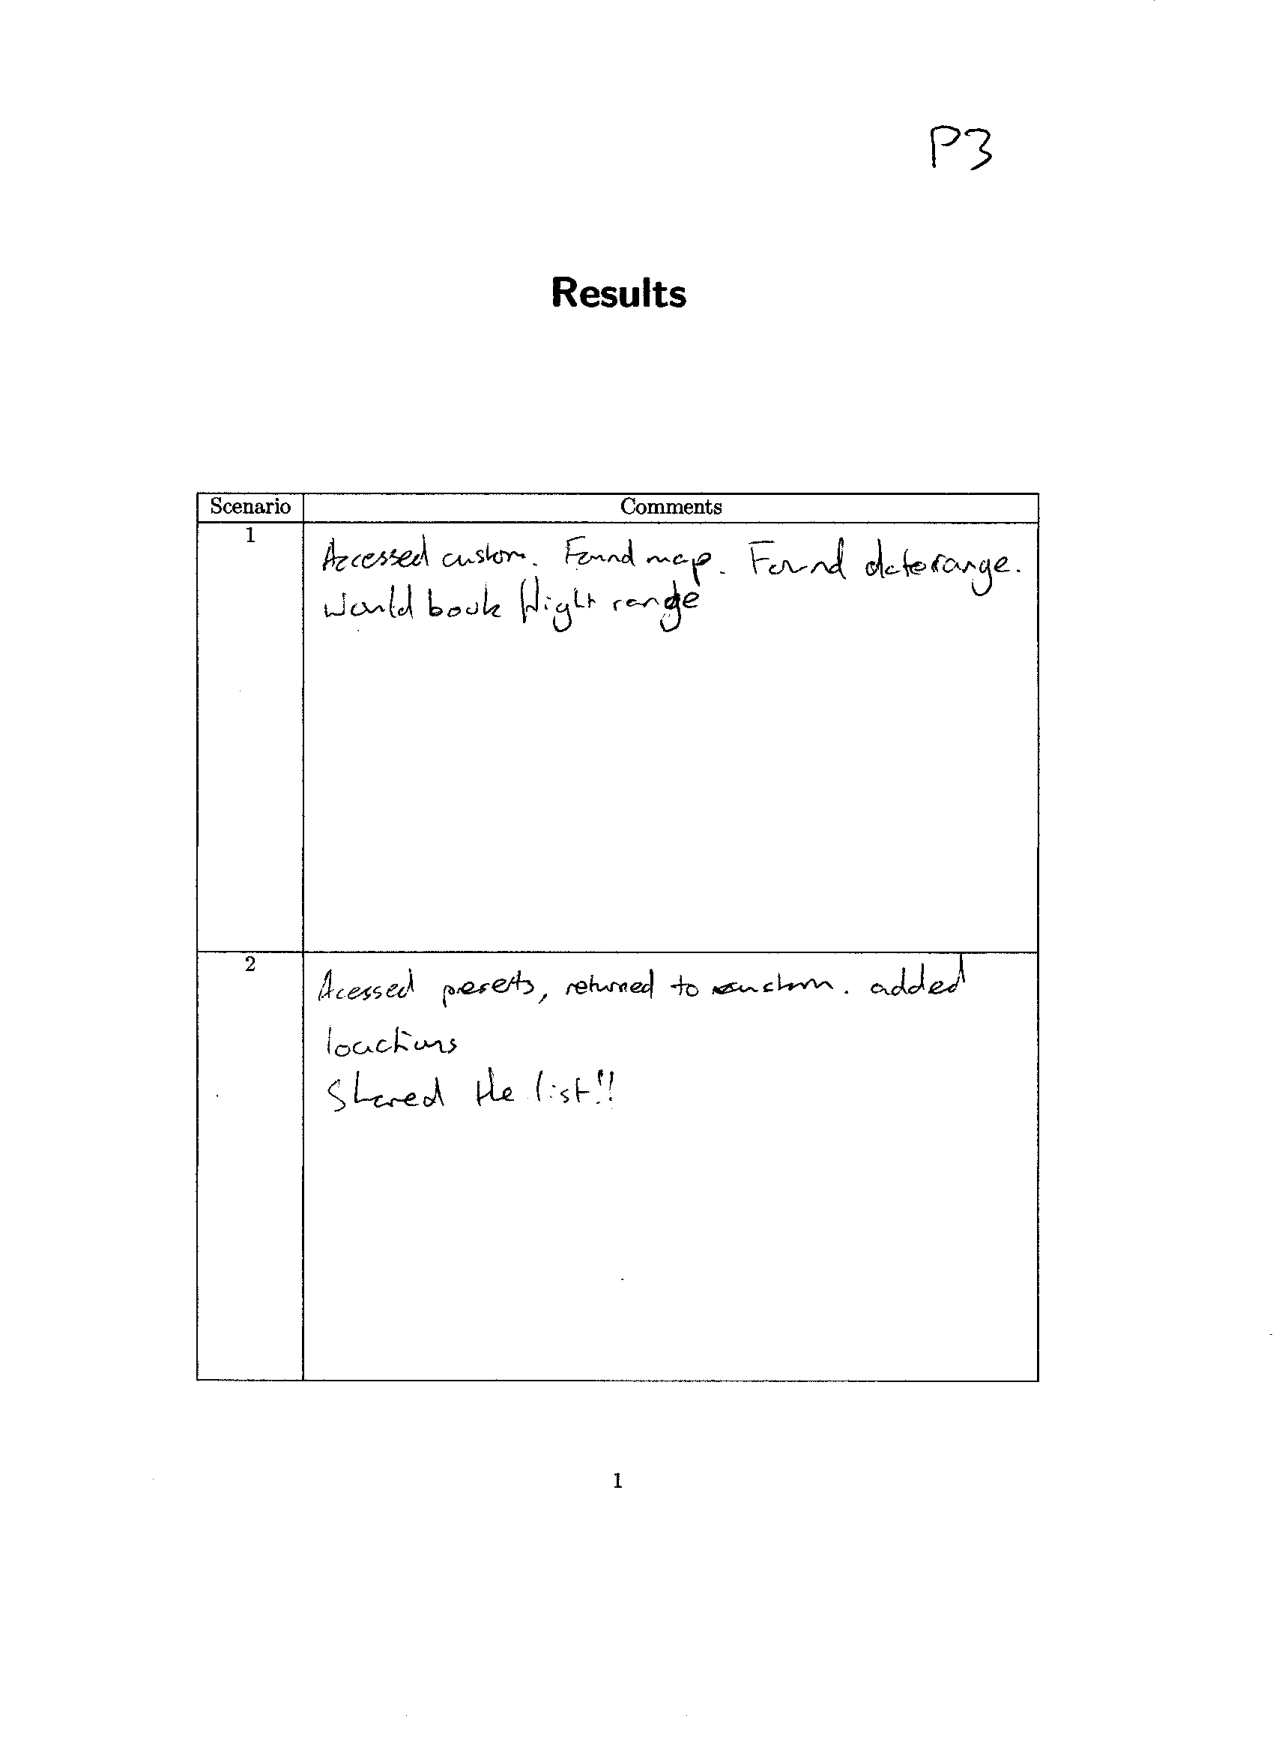
\includepdf[pages=1-2]{Results/P3-R.pdf}

\end{document}
